\chapter{Existing solutions}
In this chapter we will discuss currently available solutions in our problem domain.
First, each application is briefly introduced.
Second, we state use cases by which we later compare the applications.
Last, we describe how each application fulfills these use cases.

\section{Overview of existing similar applications}
Now we will briefly introduce available applications.

\subsection*{Allergy Menu}
There are allergen icons in the menu item's description.
A guest can interact with the menu by choosing what allergens they want to avoid.
A guest can also select an option that they are either a vegan or vegetarian.
The application filters out items of a menu to meet the guest's preferences.
The application allows a restaurant employee create a menu and specify what allergens are contained in each item of the menu.

Android and iOS app

Information on the dishes, both public and internal information can be managed along with additional documentation, such as photographs of labelling, can ensure all allergy information is logged in one place.

Our menu is designed to feel like your business, so you just upload your logo within the my account area.

You can create custom categories for your menu to help users find dishes easily.

Dished can be easily duplicated and hidden on the live system when they are not active. Allowing you to keep your menu up to date easily.

Along with the usual allergen list, there are flags to allow the system to work for vegans and vegetarians.

You can also add internal notes, recipes and method about each dish, with the ability to upload photographs of products used within a dish with notes for each photo, allowing you to manage your information easily.

When creating your recipes, it also searches product information with allergen suggestions and ingredients lists to make inputting your information easier and accurate.

\todo[inline]{write about Natasha's law in introduction - maybe in preliminaries explain legal stuff}
Print ingredient labels onto any label printer ( 54 mm x 101 mm label) or Avery labels (14 per sheet paper), quick and easily to ensure you meet Natasha's Law.

You can also download printed literature in the My Account area to create point of sale graphics for your menu with your unique reference and QR code, along with code to add a link from your website direct to the allergy menu.

The system will email you every month to review your menu with all the allergy information, you can then set if the menu is up to date, or edit from there if items have changed.

CSV import - Link up your CSV export with our system and then easily import your file as and when you need to.

API integration - Talk to your supplier about integrating with our API, allowing them to sync your information directly into Allergy Menu without manual intervention.

\begin{figure}[h]
  \centering
  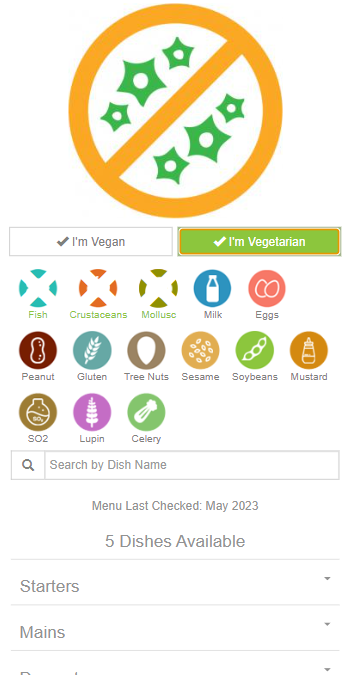
\includegraphics[width=0.62\linewidth]{master-thesis/img/allergen_menu_screenshot.png}
  \caption{The Allergy Menu application}
\end{figure}

\subsection*{Allergen Checker}


\begin{figure}[h]
  \centering
  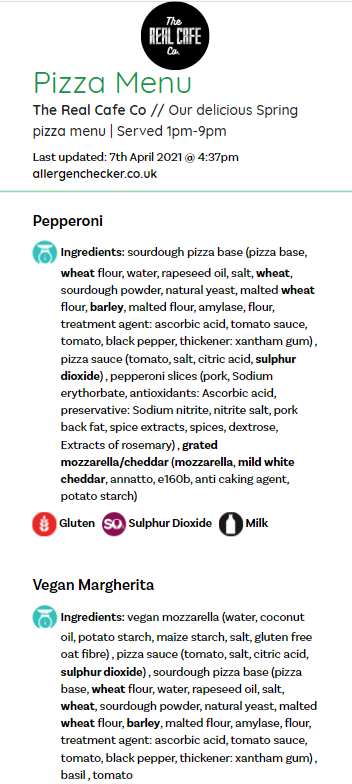
\includegraphics[width=0.62\linewidth]{master-thesis/img/allergen_checker_menu_screenshot.png}
  \caption{The Allergen Checker application}
\end{figure}

\subsection*{Tenkites}

\begin{figure}[h]
  \centering
  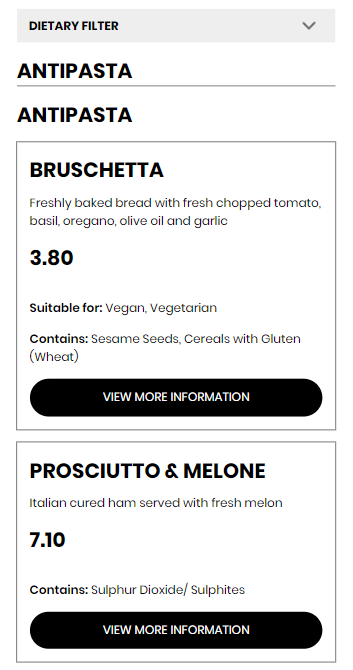
\includegraphics[width=0.62\linewidth]{master-thesis/img/tenkites_menu_screenshot.png}
  \caption{The Tenkites application}
\end{figure}

\section{Comparison of the applications}

\subsection*{Measured use cases}

\todo[inline]{add a line break in use case 9 or restructure it, so it is shorter - maybe add an option to display icons instead of allergen names}
\todo[inline]{rozdelit tabulku na dve - v jednej use casy pre hosta v druhej use casy pre restauraciu}
\begin{center}
  \begin{tabular}{| c | l |}
    \hline
    G1 & Allow a guest to create a dietary profile. \\
    \hline
    G2 & Display a personalized menu to a guest. \\
    \hline
    G3 & Allow a guest to filter out items of a menu which they cannot eat. \\
    \hline
    G4 & Display a menu after a quest scans a QR code on a printed menu. \\
    \hline
    G5 & Allow a guest to mark a restaurant as their favorite. \\
    \hline
    G6 & Allow a guest to control their personal data. \\
    \hline
    G7 & Translate a menu to the language of the UI. \\
    \hline
    G8 & Find restaurants near the guest based on their location. \\
    \hline
    G9 & Allow the guest to pay for a menu item. \\ % aplikácia umožňuje zaplatiť za účet v reštaurácii v rámci aplikácie
    \hline
    G10 & možnosť pracovať s aplikáciou neprihlásený \\
    \hline
  \end{tabular}
  \newline
\end{center}

\begin{center}
  \begin{tabular}{| c | l |}
    \hline
    R1 & Automatically add allergens to an item of a menu. \\
    \hline
    R2 & Allow a restaurant employee to choose whether to use allergen names or numbers in a menu. \\
    \hline
    R3 & Provide templates for creating a new menu. \\
    \hline
    R4 & Allow a restaurant employee to reuse a previously created menu item. \\
    \hline
    R5 & Allow a restaurant employee to control their restaurant's data. \\    
    \hline
    R6 & weights of meals \\
    \hline 
    R7 & možnosť automaticky vygenerovať menu \\
    \hline
  \end{tabular}
  \newline
\end{center}

\todo[inline]{vertically center contents of the table - may be usable for all tables in the thesis} % https://tex.stackexchange.com/questions/7208/how-to-vertically-center-the-text-of-the-cells/611601#611601
\todo[inline]{make all columns have equal width}
\subsection*{Results of the comparison}
All applications provide their guests with interactive menus which can be suited to the guests' dietary needs.

\begin{center}
  \begin{tabular}{| l | c | c | c | c | c | c | c | c | c | c|}
    \hline 
      & G1 & G2 & G3 & G4 & G5 & G6 & G7 & G8 & G9 & G10 \\
    \hline
    Choose Well & \ding{52} & \ding{52} & \ding{52} & \ding{52} & \ding{52} & \ding{52} & \ding{52} & \ding{52} & \ding{52} & \ding{52} \\
    \hline
    % App2 & \ding{52} & \ding{56} & - \\
    % \hline
  \end{tabular}
  \newline
\end{center}

\begin{center}
  \begin{tabular}{| l | c | c | c | c | c | c | c |}
    \hline 
      & R1 & R2 & R3 & R4 & R5 & R6 & R7 \\
    \hline
    Choose Well & \ding{52} & \ding{52} & \ding{56} & \ding{56} & \ding{52} & \ding{56} & \ding{52} \\
    \hline
    % App2 & \ding{52} & \ding{56} & - \\
    % \hline
  \end{tabular}
  \newline
\end{center}

\ding{52} means that an application fully supports the use case \newline
\ding{56} means that an application does not support the use case \newline
\ding{115} means that an application supports the use case only partially \newline
- means that the use case is skipped as it is out of the application's scope \newline

\todo[inline]{add Other applications worth mentioning section}
% \section{Other applications worth mentioning}
